\documentclass[french,a4paper,12pt]{report}
\usepackage[utf8]{inputenc}
\usepackage[T1]{fontenc}
%Package paramétrage:
%marge horizontale à 2,5 cm, et la marge verticale à 1,5 cm.
\usepackage{geometry}
\geometry{hmargin=2.5cm,vmargin=1.5cm}
\usepackage{graphicx}
\usepackage{float}
\usepackage{listings}
\usepackage{color}
\definecolor{dkgreen}{rgb}{0,0.6,0}
\definecolor{gray}{rgb}{0.5,0.5,0.5}
\definecolor{mauve}{rgb}{0.58,0,0.82}

\lstset{frame=tb,
  language=Java,
  aboveskip=3mm,
  belowskip=3mm,
  showstringspaces=false,
  columns=flexible,
  basicstyle={\small\ttfamily},
  numbers=none,
  numberstyle=\tiny\color{gray},
  keywordstyle=\color{blue},
  commentstyle=\color{dkgreen},
  stringstyle=\color{mauve},
  breaklines=true,
  breakatwhitespace=true,
  tabsize=3
}

\title{TR54 \\ TP Projet :\\ Intersection Autonome}
\author{Professeurs encadrants :\\LOMBARD Alexandre \\ ABBAS-TURKI Abdeljalil\\\\ Élèves :\\ROMET Pierre\\CARRION Nicolas\\BURGER Valentin\\PANASSIM Hessou}
%\hfill\hbox to 0pt{\hss\includegraphics[width=7cm]{XXXX.png}\hss}\hfill\null\newline
\date{Automne 2017}

\begin{document}

\maketitle

\tableofcontents

\part{Introduction}

\chapter{Présentation}
Dans le cadre de notre projet de TR54(Modélisation et Commandes des systèmes temps réels) nous avons choisi d'implémenter le sujet de "L'intersection autonome". Il s'agit de mettre en oeuvre un contrôle temps réel sans fil sur des "Véhicules Guidés Automatiques" (VGA), afin de gérer leur passage à une intersection et de prévenir les collisions, ceci suivant une politique prédéfinie.

\chapter{Objectif}
L'objectif du projet est la réalisation d'une intersection autonome en utilisant les robots Lego EV3.
Trois robots (ou plus) devront se déplacer sur un circuit en forme de huit et négocier leur droit de passage à
l'intersection par communication sans fil afin d'éviter les collisions.

\part{Éléments à notre disposition}
%Afin de mettre en œuvre notre projet, nous avons eu à dispositions les éléments suivants.

\chapter{Le circuit}
Le circuit mis à notre disposition est découpé en plusieurs zones:
\begin{itemize}
\item Zone d’entrée/zone de stockage (approche de l’intersection)
\item Zone de conflit (où un seul robot peut être présent)
\item Zone de sortie
\end{itemize}

\hfill\hbox to 0pt{\hss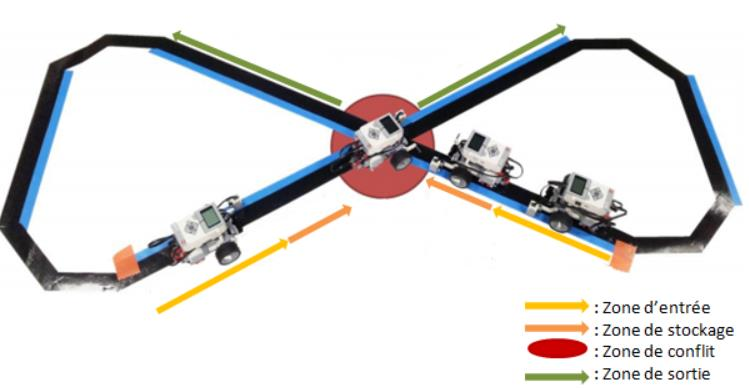
\includegraphics[width=15cm]{circuit.png}\hss}\hfill\null\newline

\chapter{Politique de négociation}
Afin de mettre en œuvre une régulation au sein de la zone d'intersection, quatre protocoles nous furent proposés (en cours et en Tp) afin d'administrer le droit de passage.

\begin{itemize}
\item Feux communicants:
Programmation horaire en donnant la couleur de feu à chaque voie (rouge/vert, rouge/rouge, vert/vert, vert/rouge).
On peut pousser l'approche pour que le robot soit au courant du temps qui reste pour obtenir le vert et ainsi adapter sa vitesse en fonction.

\item La négociation binaire:
Les véhicules arrivent dans la zone d'entrée et demandent l'accès au serveur pour son passage.
Si la zone de conflit n'est pas occupée, le robot obtient le droit de passage, sinon il est enregistré et il attend l'autorisation du serveur. Une fois la zone libérée, le serveur lui donne le droit de passage.
Une fois que le robot a fini de traverser la zone de conflit, il envoie un acquittement, afin de notifier au serveur qu'elle est libre.

\item Synchronisation de vitesse:
À l’approche de l'intersection (zone d’entrée ???? ou de stockage) un robot envoie une requête de passage au serveur.
De son côté, ce dernier construit une séquence de passage ordonnée à partir des requêtes reçues et la retransmet
à l’ensemble des robots concernés. La liste contient l’ensemble des robots ayant émis une requête pour franchir
l’intersection, leur position et leur vitesse. Tous les robots sont autorisés à franchir l’intersection, mais ils doivent synchroniser leur vitesse avec ceux qui les précèdent dans la séquence, afin que ceux-ci passent en premier. Par exemple, si un robot est en position 3 dans la séquence, il ne pourra traverser qu’après que le robot en position 2 soit sorti de la séquence. Pour ce faire, chaque robot, une fois dans la séquence de passage, doit émettre régulièrement auprès du serveur des messages pour l’informer de sa nouvelle position et sa nouvelle vitesse. Ces informations sont retransmises à
tous les robots par la séquence de passage. Tant qu’un robot n’est pas dans la séquence de passage, il doit s’arrêter avant l’intersection.

\item Synchronisation par réservation (AIM):
Cette méthode fut développée par l'université du Texas, elle consiste à ce que le véhicule estime l'horaire d'occupation de la zone de conflit afin de pouvoir demander une réservation.
Ainsi, si l'horaire est libre, le serveur l'accepte, sinon il lui refuse.
Enfin, en cas de refus, le véhicule devra retarder son horaire.
\end{itemize}

\chapter{Stratégie de régulation}
Concernant la construction de la séquence de passage, devant permettre le franchissement de la zone de conflit, deux stratégies nous furent proposées:

\begin{itemize}
\item FIFO (first-in first-out) : 
	Le premier arrivé à l’intersection est le premier à en sortir, dans le cadre de cette
	politique, un soin particulier devra être apporté à la prévention des situations d’interblocage
	
\item Batch : lorsqu’un robot se présente à l’intersection, il est ajouté à la séquence de passage, si et
	uniquement si, l’une des deux conditions suivantes est remplie :
	\begin{itemize}
	\item La séquence de passage actuel est vide
	\item Le dernier robot dans la séquence de passage provient de la même voie que le robot actuel
	\item Le dernier robot dans la séquence de passage provient de l’autre voie, mais le délai entre l’ajout
		de ce dernier robot et du robot courant est supérieur à un seuil dT (par exemple 5 secondes)
	\end{itemize}
\end{itemize}


\part{Travail Réalisé}

\chapter{UML}

\section{Diagramme de classes}
Nous avons construit notre projet selon les diagrammes de classes suivants:\newline

\hfill\hbox to 0pt{\hss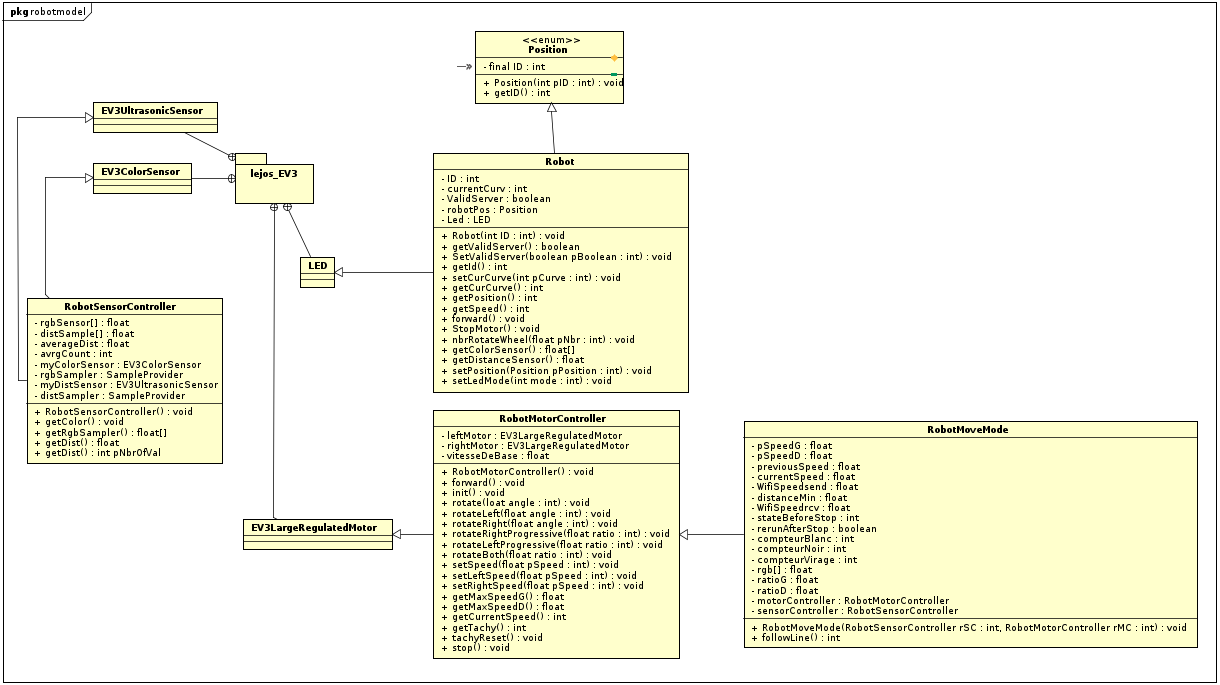
\includegraphics[width=20cm]{robotmodel.png}\hss}\hfill\null\newline

\hfill\hbox to 0pt{\hss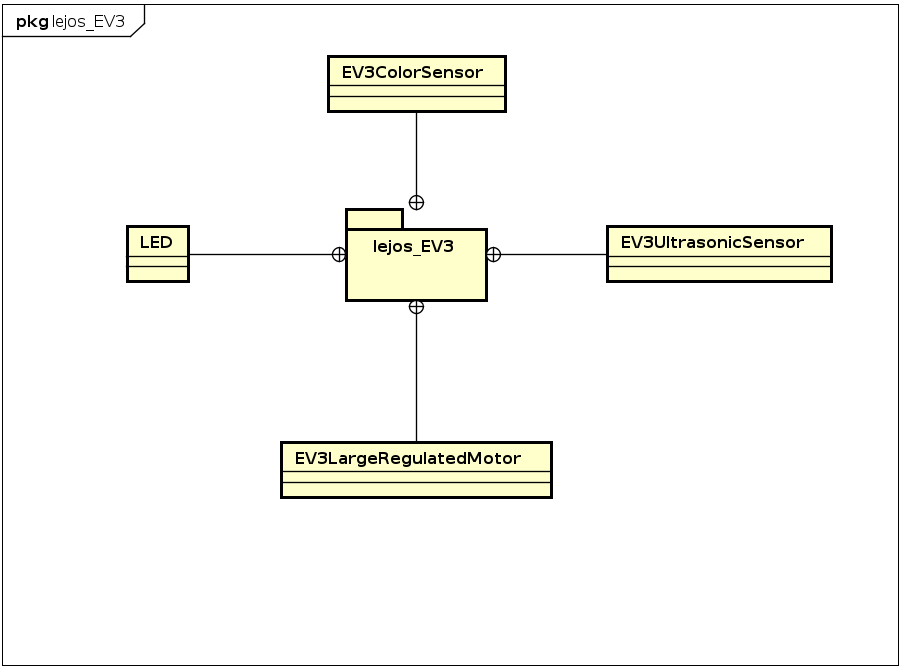
\includegraphics[width=15cm]{lejos_EV3.png}\hss}\hfill\null\newline

\hfill\hbox to 0pt{\hss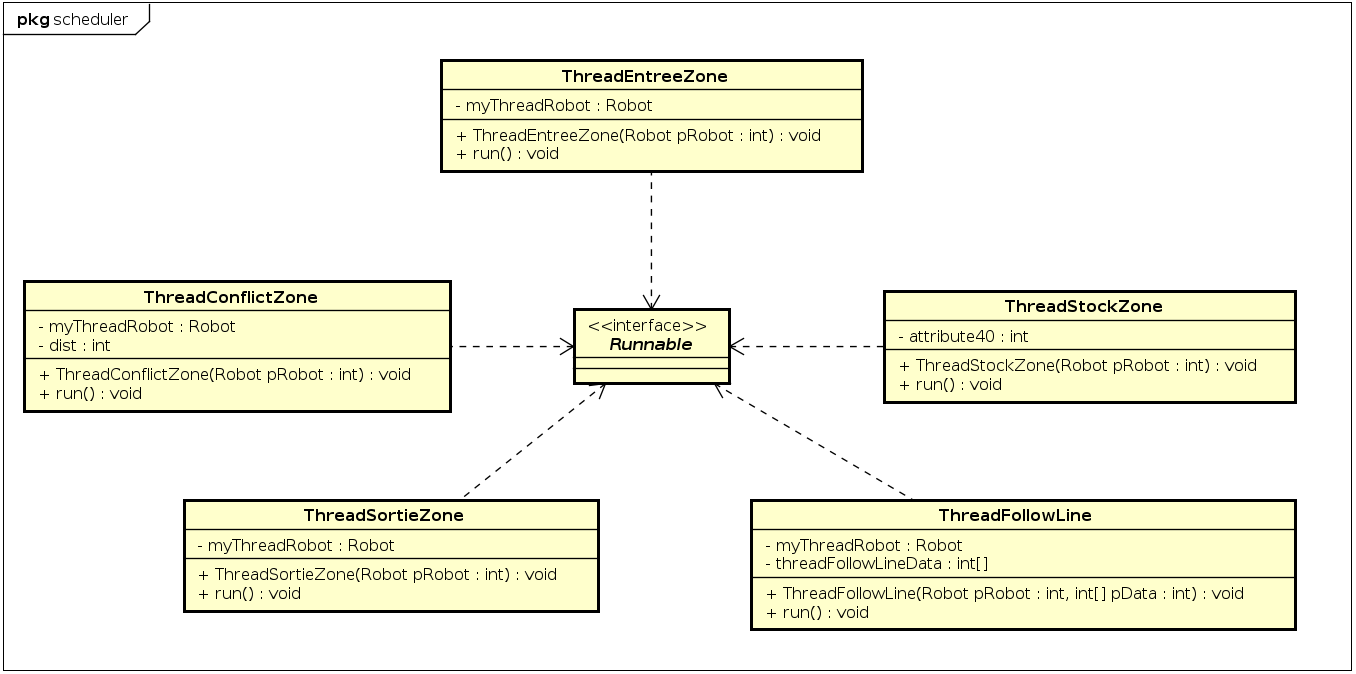
\includegraphics[width=20cm]{scheduler.png}\hss}\hfill\null\newline

\hfill\hbox to 0pt{\hss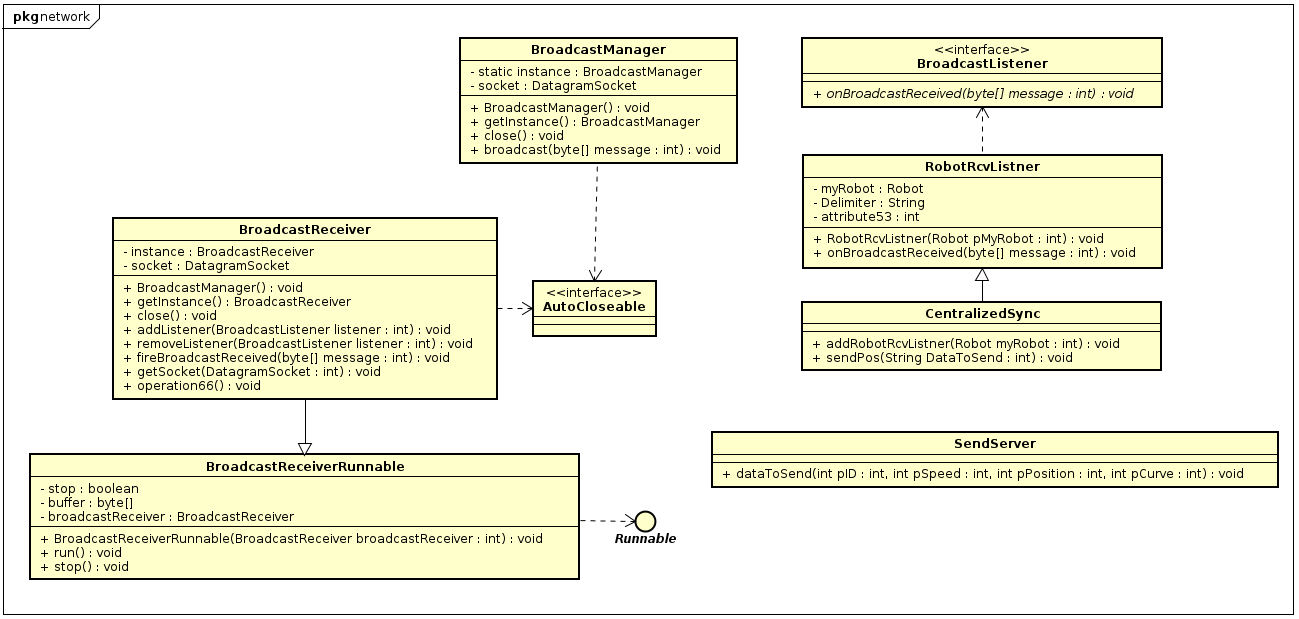
\includegraphics[width=21cm]{network.png}\hss}\hfill\null\newline

\hfill\hbox to 0pt{\hss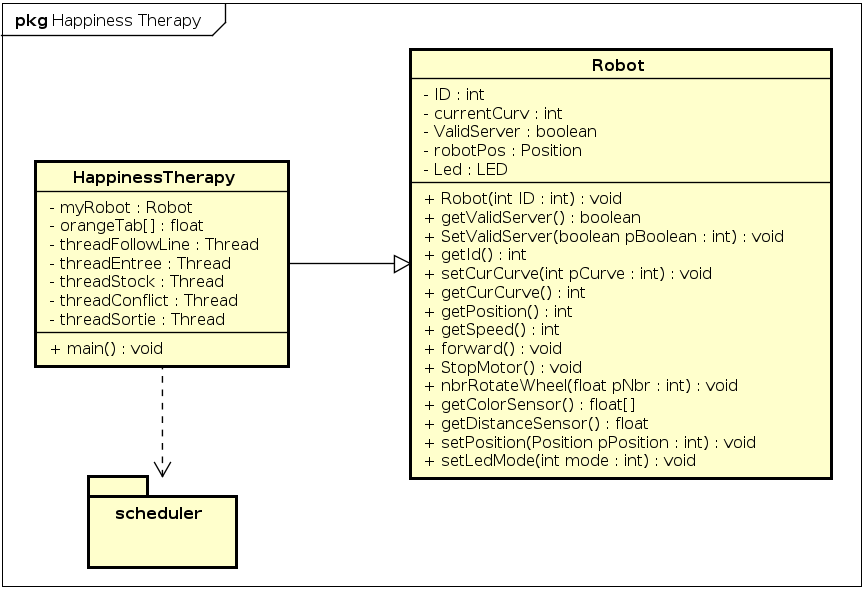
\includegraphics[width=21cm]{HappinessTherapy.png}\hss}\hfill\null\newline

\section{Diagramme de séquence}

Afin de décrire les échanges entre les robots et le serveur, lors de la détection de la marque orange, ainsi qu'à l'entrée dans la séquence de passage, nous avons réalisé le diagramme de séquence suivante:

\hfill\hbox to 0pt{\hss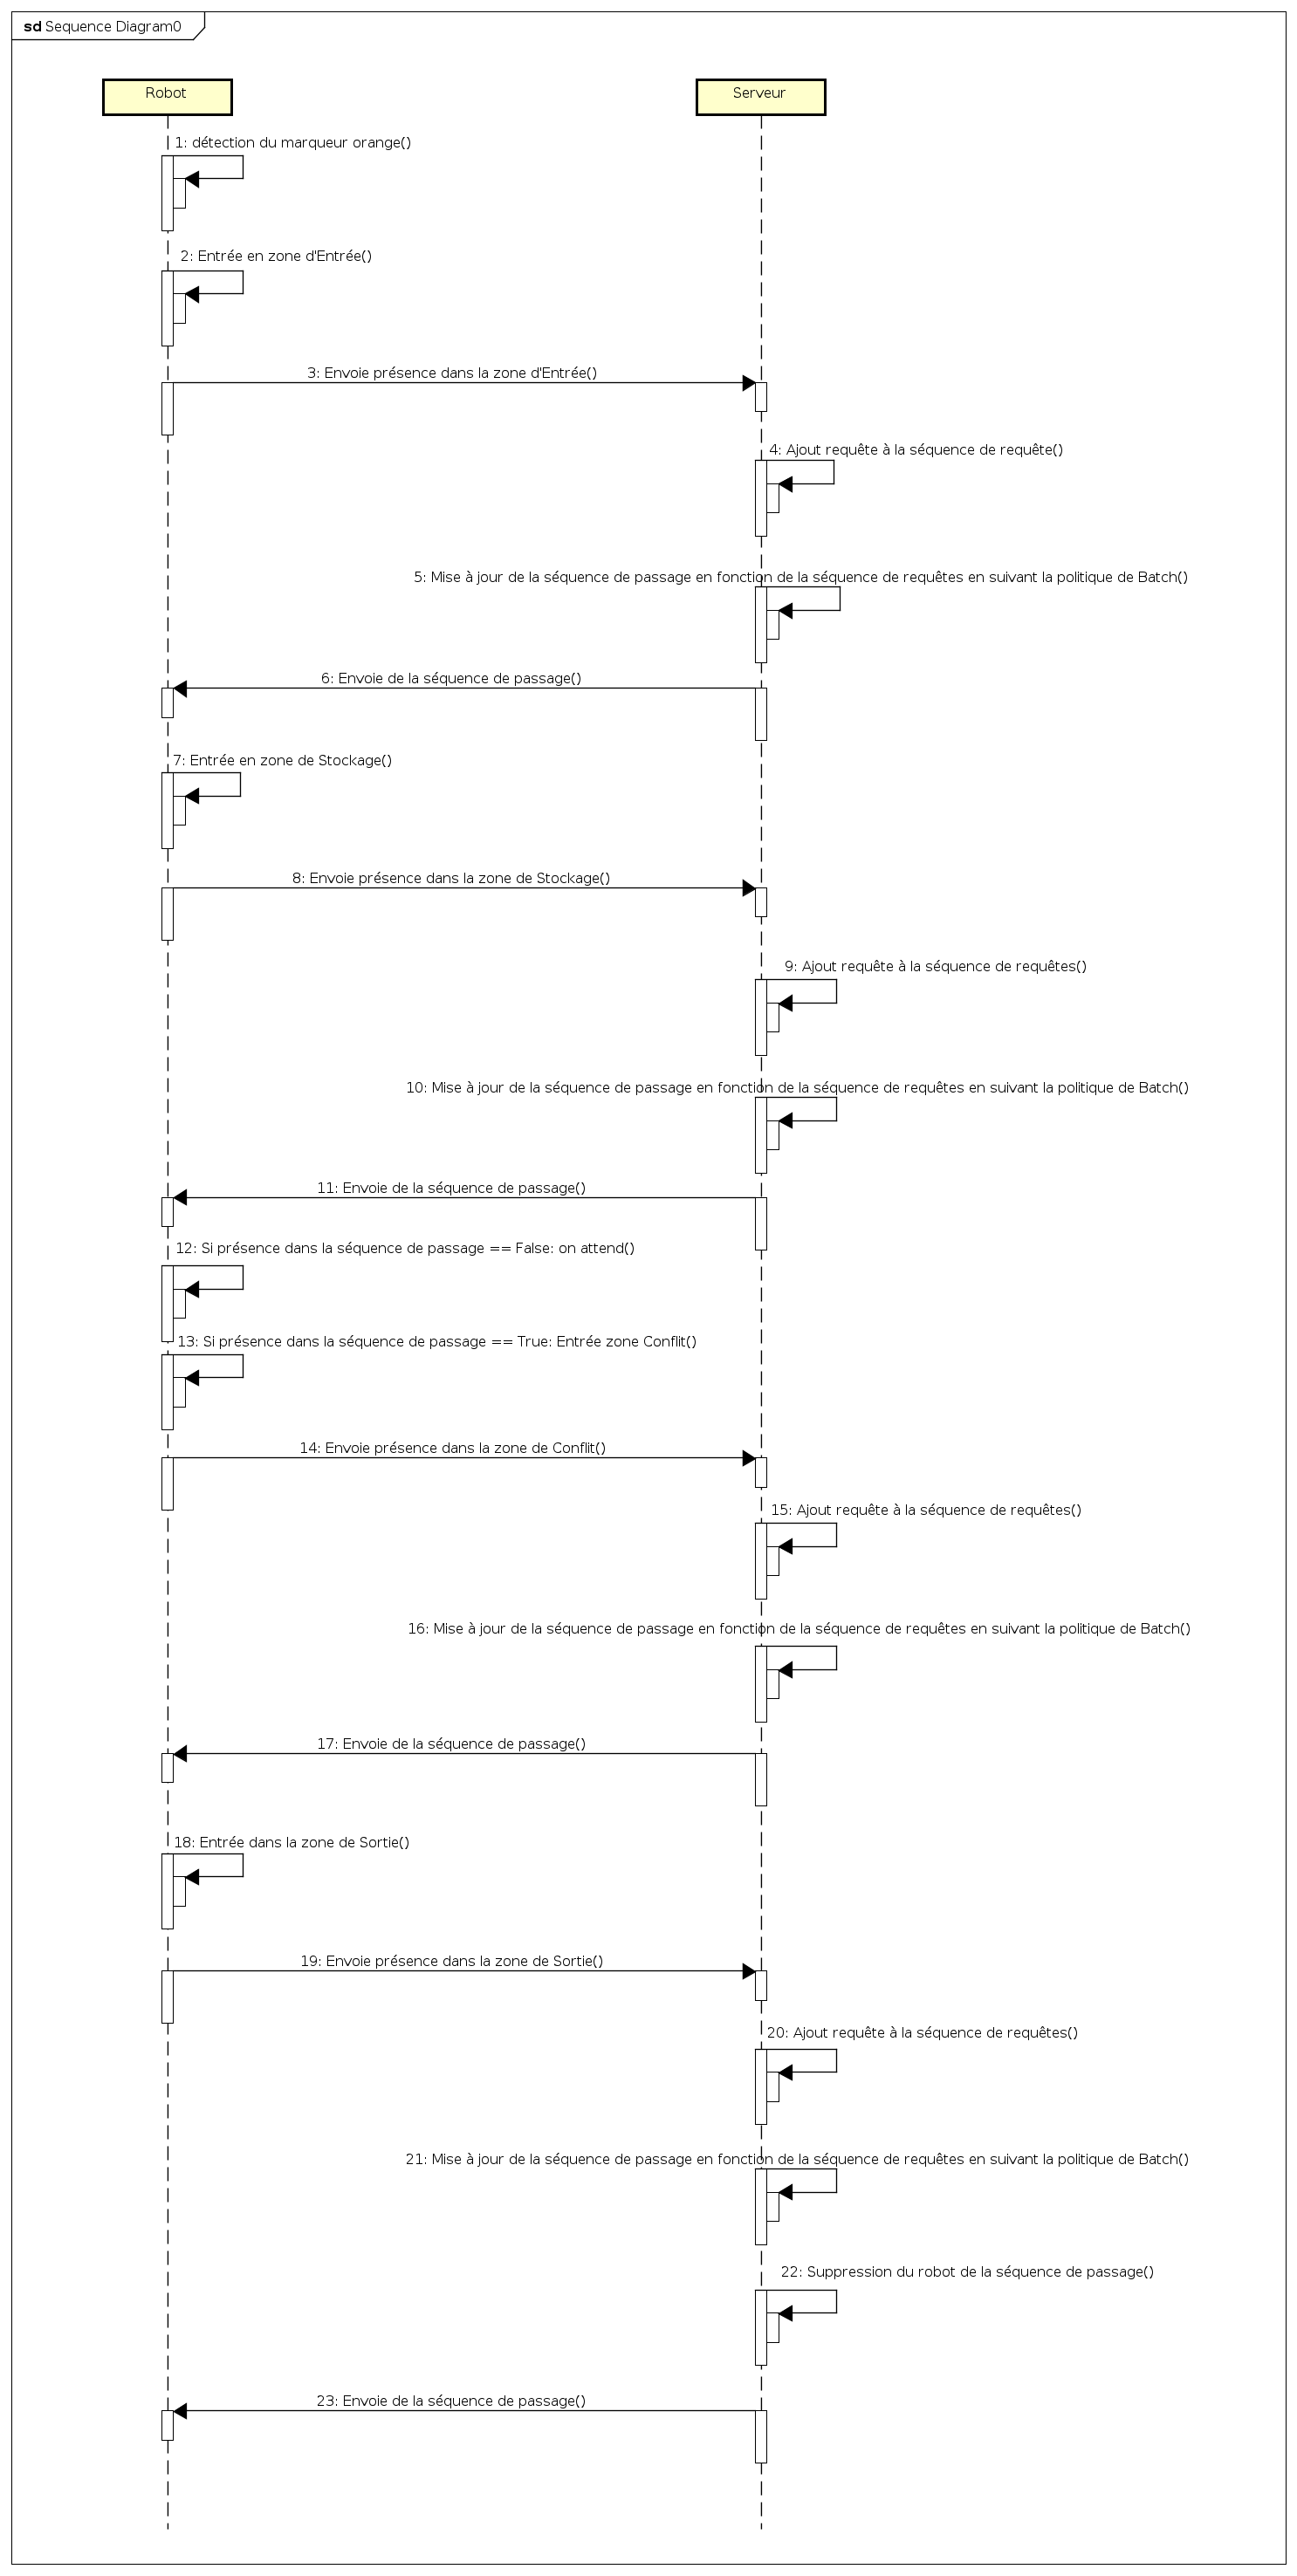
\includegraphics[width=11cm]{diagSeq.png}\hss}\hfill\null\newline


\chapter{Intersection}

\section{Politique de négociation}
La politique de négociation utilisée pour notre projet, afin de gérer le droit de passage des robots au sein de la zone de conflit, est la politique de synchronisation des vitesses. Bien que cette politique ait été imposée par le sujet, elle offre une méthodologie plus complète que les autres politiques présentés plus tôt dans ce chapitre.

En effet, on retrouve la gestion via un serveur centralisé, mais qui offre un mécanisme plus sophistiqué, en utilisant plusieurs zones de contrôle. De plus, une communication inter-robot afin d'adapter la vitesse de déplacement entre les robots au sein des zones offre une méthodologie plus élégante.

\section{Stratégie de régulation}
Pour ce projet, deux stratégies de régulation nous furent proposées.
Nous avons choisi d'implémenter la politique de "BATCH",la jugeant plus performante, après analyse.

Le principal inconvénient de la stratégie "FIFO", réside dans son utilisation de l'horloge.
En effet, dans le cas où deux robots se présentent quasiment au même instant pour franchir la zone d'intersection, si l'un des messages transmis est perdu, compromis ou envoyé en retard alors il y a un risque que le deuxième robot s'engage dans la zone de conflit alors que le premier est déjà en train de la franchir.

De plus, cette stratégie ne tient pas compte du nombre de robot dans une section pour donner la priorité de passage. Ainsi, il peut se produire un cas d'engorgement sur une zone, sans que cette dernière ne puisse évacuer ces occupants.

La politique de "BATCH" étant certes plus complexe, a l'avantage de pallier ces deux problèmes, en couvrant plus précisément les situations de conflit ou d'interblocages.

\chapter{Communication sans fil}---
Comme nous l'avons vu dans le chapitre précédent, la communication sans fil est au cœur même de notre projet. En effet, s'est elle qui nous permet de mettre en place notre politique de négociation et notre stratégie de régulation.
La communication sans fil se base sur une connexion Wi-Fi, client/serveur, avec un échange évoluant autour d'une synchronisation centralisée des données.

La communication sans fil est donc divisée en deux parties:

\section{Partie Client (robot Lejos EV3)}%Pierre
Comme nous l'avons vu précédemment, si nous voulons pouvoir mettre en place une politique de négociation et une stratégie de régulation, il va nous falloir échanger des données clefs entre les robots, et le serveur.

Pour cela, nous avons mis en place une communication basée sur le protocole TCP/IP, devant nous permettre de certifier l'envoi des données. Le protocole TCP étant orientée-connexion par le principe de la poignée de main (handshake), il établit au préalable une connexion entre les processus avant de débuter la transmission.

Nous échangeons ainsi entre le robot et le serveur, une structure de données regroupant:
  \begin{itemize}
  \item L'identifiant du robot envoyant les données.
  \item La vitesse actuelle du robot en déplacement.
  \item La zone dans laquelle le robot évolue (zone entrée, stockage, conflit et sortie).
  \item La virage, du quel le robot provient, afin de permettre au serveur de déterminer de quel côté le robot se présente, afin de franchir la zone de conflit.
  \end{itemize}
  
Les données sont transmises sous la forme d'une chaine de caractères afin de pouvoir être envoyé tels qu'une séquence de contrôle; nous l'avons basé sur le modèle suivant:

\hfill\hbox to 0pt{\hss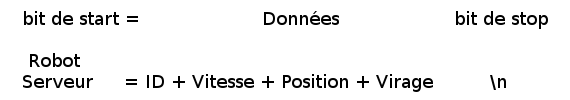
\includegraphics[width=10cm]{sequ.png}\hss}\hfill\null\newline

Ainsi, la même séquence de contrôle pourra être utilisé pour transmettre les informations du serveur au robot.

Il ne lui reste plus qu'à être traité par le serveur, pour utiliser les données.

\section{Partie Serveur}%Valentin

Pour ce projet, concernant le type de serveur utilisé, nous nous sommes porté sur un serveur Java tournant sur machine Linux ou Windows.
Nous avons choisi ce type de serveur, car il nous a permis de contourner les difficultés rencontrées par le premier type de serveur que nous avions choisi d'utiliser; le eobot Lejos EV3.
La principale difficulté étant que l'utilisation du Wi-Fi sur les robots reste très aléatoire, quant à arriver à le connecté à un hotspot. De plus, cela nous à permis de nous séparer de la contrainte matériel, nous permettant de développer le serveur et de réaliser des tests en dehors des heures de Tp.

Le serveur utilisé dans ce projet est un serveur fonctionnant avec le protocole UDP. Son rôle ici est de centraliser les messages des différents robots présents sur le circuit afin de déterminer un ordre de passage dans l’intersection, c’est-à-dire en donnant ou en ne donnant pas l’autorisation de franchir l’intersection à chaque robot.

Le serveur fonctionne en 3 parties majeures. La première partie concerne la réception et l’enregistrement des données envoyées par les robots. La seconde partie se chargera de construire la séquence de passage en fonction des requêtes reçues et en suivant la politique batch expliquée plus haut. Pour finir, le serveur envoie cette séquence de passage à l’ensemble des robots qui n’auront qu’à vérifier s’ils sont présents dans la liste. Si oui alors ils peuvent avancer, sinon, ils attendent les prochaines instructions.

L’implémentation finale utilisée fonctionne sur un ordinateur, même si elle peut être portée sur un robot. Du point de vue du code elle fonctionne de la manière suivante.

On crée un listener qui va se déclencher à chaque réception d’un message sur le réseau via le protocole UDP. À partir de se listener, les données vont être converties de Bytes à String afin de pouvoir traiter les données plus facilement. Les données sont ensuite traitées comme suit :

Voici un exemple de trame de données provenant d’un robot: " 0\textbackslash n0 \textbackslash n255 \textbackslash n-1 " \newline

\hfill\hbox to 0pt{\hss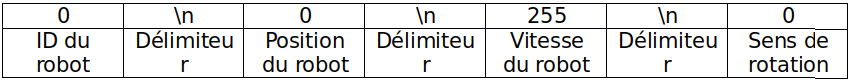
\includegraphics[width=15cm]{val.png}\hss}\hfill\null\newline

Une fois la trame de données reçues, elle est découpée suivant les délimiteurs afin de former un couple de 4 variables rassemblant ainsi, la position, la vitesse et le sens de rotation d’un robot défini par son ID. À cela, on ajoute le temps système du serveur afin de gérer la dimension temporelle des demandes. On prend ici le temps serveur, car c’est une base commune à tous les robots.

Une fois tout ceci effectué, on passe à la partie mise à jour de la séquence de requête. En effet, chaque robot effectuant une requête ne se retrouve pas directement dans la séquence de passage, c’est pourquoi il faut une séquence « tampon » afin de conserver les demandes. Il se présente alors 2 cas :
\begin{itemize}
\item Le robot est déjà présent dans la liste
	On met à jour sa position, sa vitesse ainsi que son sens de rotation
	
\item Le robot n’a pas été trouvé dans la liste
	On l’ajoute à la liste
\end{itemize}

Quand la séquence de requête est à jour, on passe à la création de la séquence de passage. Celle-ci est créée conformément à la politique batch. C’est-à-dire :
\begin{itemize}
\item Si la séquence de requête ne comporte qu’un robot et que la séquence de passage est vide.
	Ajouter le robot dans la séquence de passage
	
\item Sinon on parcourt la séquence de requête

\item Si un robot de la séquence de requête est présent dans la séquence de passage
	\begin{itemize}
	\item Si le robot a quitté l’intersection
		On le retire de la séquence de passage
		
	\item Sinon
		On met à jour sa position, sa vitesse ainsi que son sens de rotation
	\end{itemize}
	
\item Sinon, si le robot n’a pas été trouvé dans la séquence de passage
	\begin{itemize}
	\item Si le dernier robot présent dans la séquence de passage à le même sens de rotation que le robot actuel
		Ajouter le robot à la séquence de passage
		
	\item Sinon, si le délai entre la requête du dernier robot et du robot actuel excède un certain seuil (deltaTime)
		Ajouter le robot à la séquence de passage
	\end{itemize}	
\end{itemize}

Pour finir, le serveur se charge de créer une string représentant l’ensemble de la séquence de passage en y ajoutant un identifiant (« -1 ») en début et fin de chaîne afin de permettre aux robots de différencier les messages provenant du serveur des messages provenant des autres robots.

La séquence de passage est donc composée de ces deux identifiants, ainsi que des IDs, positions et vitesses des robots autorisés à franchir l’intersection. 

Une fois créée, cette séquence ressemble à celle-ci: " -1 \textbackslash n0 \textbackslash n0 \textbackslash n255 \textbackslash n[…] \textbackslash n-1 " \newline
 

\hfill\hbox to 0pt{\hss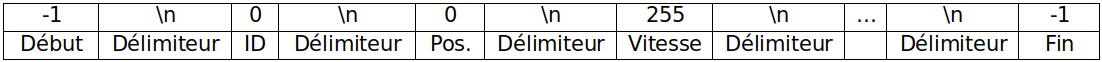
\includegraphics[width=15cm]{val2.png}\hss}\hfill\null\newline

\chapter{Franchissement des zones de contrôles}
Comme expliqué dans la partie précédente, le franchissement des zones de contrôle est rendu possible par la communication sans fil (Wi-Fi) que nous venons de voir. De plus, un échange standardisé est mis en place de façon à disposer de même design, quant au format utilisé pour échanger les données entre les robots et le serveur et inversement.

Nous allons voir dans cette partie, comment nous avons implémenté la synchronisation de vitesse, ainsi que la politique de "Batch".

Comme illustré par le diagramme de séquence, à l'approche de l'intersection (ou zone d'entrée), le robot va émettre les données( que nous avons présentées plus tôt) au serveur, puis va s'engager dans cette zone.
Ensuite, le robot va arriver dans la zone de stockage où il va à nouveau émettre les mêmes données, actualisé à destination du serveur.

Dans un même temps, la stratégie de régulation est mise en œuvre. Lorsque le robot entre dans la zone de stockage, il va commencer à attendre un acquittent du serveur, lui spécifiant qu'il peut ou non, traversé la zone de conflit. Dans le cas où cet acquittement est négatif, le robot cessera alors d'avancer pour attendre que son acquittement soit validé. Dans le cas contraire, le robot va s'engager dans la zone de conflit, mais si un autre robot est présent en sortie de zone, ce dernier va le détecter grâce à l'utilisation du capteur de distance et ainsi ralentir et franchir la zone.

Ensuite, le robot franchira la zone de sortie, qui une fois dépassé, nous permettra de retirer le robot de la séquence de passage.

Il est également à remarquer, qu'il nous fut proposé d'ajouter un contrôle visuel (à l'aide de LED) afin de nous assurer que la séquence de passage est valide. Le premier robot dans cette séquence affichera une couleur verte, le deuxième une couleur orange et à partir du troisième une couleur rouge sera utilisée.

\chapter{Le suivi de ligne} %Nico && Nadège

\section{Méthode utilisée}
Notre méthode de suivi de ligne consiste à suivre la bordure gauche du chemin, en alternant entre le blanc et le noir. Le robot diminue progressivement la vitesse d’une de ses roues (gauche ou droite selon la rotation voulue) dans l’objectif d’avancer tout en tournant, et va tout droit lorsqu’il est dans le bleu.

Afin de ne pas rester bloqué dans l'un r des deux couleurs, nous avons adopté une dégression progressive de la vitesse de la roue concernée. En d'autres termes, plus le robot reste dans une même couleur, plus la rotation augmente, avec pour objectif de ne pas trop s'éloigner de la bordure.

Nous diminuons la vitesse du moteur de la roue gauche si nous voulons tourner à gauche, à l’inverse, nous diminuons la vitesse du moteur de la roue droite si nous voulons tourner à droite. La vitesse de la roue concernée évolue selon la fonction suivante :

Vitesse = C * i * vitesse initiale

Avec :
\begin{itemize}
\item "C" est un coefficient égal à 0.95 (pour la rotation à gauche) et 0.96 (pour la rotation à droite).

\item "i" le nombre d’itérations durant lesquels le robot se trouve dans une même couleur.
\end{itemize}

Vu que "C" est inférieur à 1, la vitesse diminuera progressivement jusqu’à 0.
Nous avons des coefficients différents cars nous avons observé, par tâtonnement, un comportement anormal lorsque le coefficient était égal à 0.95 pour les 2 rotations.

\section{Détection virage précédent}
Dans le but de connaître la zone de stockage dans laquelle se trouve chaque robot. Nous avons implémenté un compteur permettant de connaître le sens du virage précédant l’entrée dans la zone de stockage.
Ce compteur suit la logique suivante :
\begin{itemize}
\item Remis à zéro lorsque le robot est dans le bleu

\item Incrémentation lorsque le robot est dans le noir

\item Décrémentation lorsque le robot est dans le blanc
\end{itemize}

Lorsque le robot passe sur les marqueurs orange (correspond à l’entrée du robot dans une zone d’entrée), si le compteur est positif cela équivaut à dire que le virage précédent était un virage à gauche. Inversement si le compteur est négatif, cela équivaut à dire que le virage précédent était un virage à droite.

\part{Analyse critique}

\chapter{Difficultés rencontrées \& Solutions apportées}

\section{Partie serveur}
Au début du projet, l’idée fut de partir sur une implantation du serveur, au cœur du même code que la partie client pour les robots afin de ne travailler que sur un projet global.

Cette contrainte imposait donc uniquement l’utilisation des robots pour le serveur, ce qui d’une part n’était pas très pratique pour la connexion (comme la connexion Wi-Fi était un peu aléatoire).
D’autre part, cela nous contraignait à ne pouvoir réaliser des tests uniquement lorsque les robots étaient à notre disposition ; nous empêchant donc de travailler depuis chez nous.

La solution qui a été mise en place fut de dissocier le code serveur et le code client, afin de pouvoir faire tourner le serveur sur n’importe quelle plateforme (aussi bien sur un robot que sur une machine Linux ou Windows).
Enfin, cette solution nous a permis de pouvoir effectuer des tests via l'outil "Netcat", afin de simuler des envois de données provenant de robots dans un environnement isolé.

\section{Suivi de ligne}
La principale difficulté quant au suivi de ligne reste la détection des couleurs. Il nous avait été proposé de travailler avec les données brutes du capteur RGB, mais au final, l'utilisation de données, traité au préalable par la brique Lejos, c'est avéré nous apporter plus de souplesse dans la détection des couleurs.
\newpage

\chapter{Conclusion}
Lors de ce Tp, il nous fut demandé de réaliser une intersection autonome en utilisant les robots Lejos EV3.

Pour cela, nous avons dû mettre en place les structures suivantes:
\begin{itemize}
\item Une communication sans fil, basée sur le Wi-Fi.

\item Une politique de négociation ainsi qu'une stratégie de régulation

\item Un algorithme nous permettant de suivre le parcours d'un circuit.
\end{itemize}

Vis-à-vis de la communication sans fil, bien que les robots soient dotés de Wi-Fi, l'utilisation de ce dernier reste extrêmement handicapant, du fait de son côté aléatoire.
Concernant notre serveur, ce dernier est fonctionnel, mais adapté à une structure de données de petite taille, même si certains aspects seraient exactement les mêmes à grande échelle. Cependant, il reste certains points qui pourraient ne pas fonctionner. 
En effet, les traitements effectués par le serveur s'effectuent dès lors d'une réception de données. Le problème qui ainsi, peut se poser, est que les listes de requêtes et de passage étant de grande taille, elles seront très longues à explorer, ce qui induit un temps de traitement supérieur au temps entre deux réceptions de message, ce qui pourrait causer des problèmes d'accès à des ressources partagées.
Pour pallier ce problème, il nous suffirait d’implémenter des threads utilisant des exclusions mutuelles (mutex), pour accéder aux ressources critiques. Cette solution n’a pas été retenue car jugée trop "lourde" dans le cas de cette structure.
Une autre méthode, afin de manager de grandes structures de données en tenant compte de priorités, aurait pu être implémentée au travers de "TAS Max".

Concernant le suivi de ligne, bien que l'algorithme utilisé soit totalement fonctionnel, un problème handicapant persiste, la couleur. En effet, la brique Lejos nous permet de détecter les couleurs, ce qui nous est indispensable. Cependant, il s'avère que les couleurs évoluent, changent au cours de la journée en fonction de la quantité de lumière. Nous obligeant à devoir, lors de chaque séance, effectuer un nouvel échantillonnage des couleurs, afin que les robots puissent suivre le parcours sans dévier.

Afin de continuer à faire évoluer le projet, nous avons pensé qu'il serait intéressant de développer les parties suivantes:
\begin{itemize}
\item Au long du semestre, nous avons travaillé sur un circuit donné; il serait cependant intéressant de savoir si le protocole développé reste fonctionnel, si le circuit venait à changer, en ayant des zones de conflits plus complexes.

\item De plus, utilisant plusieurs robots, avec des IDs différents, nous devons actuellement les paramétrer à la main. Une solution envisageable, serait d'implémenter une discussion entre les robots, afin qu'ils se découvrent et s'attribuent eux-mêmes des identifiants.
\end{itemize}

\end{document}
